\documentclass[journal]{IEEEtai}

\usepackage[colorlinks,urlcolor=blue,linkcolor=blue,citecolor=blue]{hyperref}

\usepackage{color,array}
\usepackage{booktabs}

\usepackage{graphicx}
\usepackage{amsthm}
\usepackage{algorithm}
\usepackage{algpseudocode}
\usepackage{xspace}
\usepackage{amsmath,amssymb}

\newcommand{\pending}{\textemdash}
\newcommand{\hsfp}{H-SFP\xspace}
\newcommand{\ehsfp}{E-HSFP\xspace}

\newcommand{\pmu}{\mu}
\newcommand{\psigma}{\sigma}
\newcommand{\mem}{\mathcal{M}}
\newcommand{\stale}{\tau}
\newcommand{\dropoutp}{p}
\newcommand{\drift}{{\Delta_{\mathrm{proto}}}}
\newcommand{\clients}{\mathcal{C}}
\newcommand{\classidx}{j}
\newcommand{\edgeidx}{m}
\newcommand{\memcap}{M_{\mem}}

\newtheorem{theorem}{Theorem}
\newtheorem{lemma}{Lemma}
\newtheorem{assumption}{Assumption}
\newtheorem{corollary}{Corollary}
\newtheorem{definition}{Definition}
\newtheorem{remark}{Remark}


%% \jvol{XX}
%% \jnum{XX}
%% \paper{1234567}
%% \pubyear{2020}
%% \publisheddate{xxxx 00, 0000}
%% \currentdate{xxxx 00, 0000}
%% \doiinfo{TQE.2020.Doi Number}

\setcounter{page}{1}
%% \setcounter{secnumdepth}{0}


\begin{document}


\title{E-HSFP: Episodic Hierarchical Split-Federated Prototyping\\
A Serverless-Aware Learning Framework for Stateless Cloud--Edge Training} 


\author{Author~One, Author~Two, and Author~Three%
\thanks{% TODO(meta): confirm author list and affiliations before submission.
Author affiliations and funding acknowledgments will be added before submission.}}

\markboth{Journal of IEEE Transactions on Artificial Intelligence, Vol. 00, No. 0, Month 2020}
{Author One \MakeLowercase{\textit{et al.}}: E-HSFP: Episodic Hierarchical Split-Federated Prototyping}

\maketitle
\begin{abstract}
Federated learning enables collaborative model training without centralizing raw data, but practical deployment remains challenging under statistical heterogeneity, resource-constrained clients, and unstable intermediate computation. Split federated learning reduces client-side computation by partitioning neural networks across clients and servers. However, existing split federated methods usually preserve an end-to-end optimization graph, requiring continuous transmission of smashed activations and cross-tier gradients. This creates high communication cost and tight synchronization dependencies, making convergence difficult to guarantee under partial, stale, or asynchronous updates.
In this paper, we propose Episodic Hierarchical Split-Federated Prototyping (E-HSFP), a convergence-guided extension of hierarchical split-federated prototyping. Instead of treating serverless-style execution as a resource allocation problem, we study it as a learning problem where upper-tier models optimize over incomplete and temporally shifting prototype-induced feature distributions. E-HSFP introduces episodic prototype memory, reliability-aware prototype aggregation, prototype dropout regularization, prototype replay consistency, and a residual prototype generator to control prototype-induced distributional drift.
The main theoretical contribution is a convergence analysis for decoupled hierarchical split-federated learning under partial prototype updates, stale prototype updates, and episodic prototype updates. We decompose the convergence error into stochastic gradient noise, periodic sub-model aggregation divergence, partial prototype updates, stale prototype updates, memory replay error, and synthetic distribution approximation error. Under standard smoothness, bounded variance, and measure-Lipschitz assumptions, the target result is a convergence guarantee to a stationary neighborhood whose radius is controlled by prototype-induced distributional drift. We evaluate image classification and medical segmentation under IID and non-IID partitions, missing and stale prototype packets, and simulated serverless disruptions. Under a matched 60-round, five-seed protocol with 200 clients, E-HSFP improves on H-SFP by 3.71, 3.19, and 25.80 accuracy points on CIFAR-10, CIFAR-100, and HAM10000 while using slightly less communication, and it limits accuracy loss under prototype dropout and serverless-style disruptions to at most 1.81 points. Under this protocol, however, both prototype-based methods trail the strongest weight-sharing baselines in classification, and E-HSFP does not improve ISIC-2018 segmentation over H-SFP.
\end{abstract}

\begin{IEEEImpStatement}
% TODO(meta): replace with the final IEEE TAI impact statement before submission.
This extension studies how hierarchical split-federated learning can remain stable when cloud--edge training is episodic, asynchronous, and driven by incomplete prototype summaries.
\end{IEEEImpStatement}
\begin{IEEEkeywords}
Federated learning, split learning, hierarchical federated learning, prototype learning, convergence analysis, asynchronous optimization, serverless computing.
\end{IEEEkeywords}
\section{Introduction}
Federated learning (FL) has become a standard paradigm for collaborative model training without centralizing raw data, with FedAvg~\cite{mcmahan2017communication} and heterogeneity-aware extensions such as FedProx~\cite{li2020federated} establishing the modern optimization framework for decentralized learning under communication and systems constraints. Yet, even in this mature line of work, convergence remains fragile when clients are statistically heterogeneous, intermittently available, or resource-constrained, because the global objective is optimized through delayed and imperfect local surrogates rather than through direct centralized gradients. This tension is especially acute when the model is too large or too expensive to train fully on-device, motivating alternatives that reduce client-side memory, computation, and communication while preserving privacy. 

Split learning (SL) offers one such alternative by partitioning a neural network across clients and servers so that clients compute only shallow layers while deeper layers are executed remotely~\cite{vepakomma2018split}. Hierarchical client-edge-cloud variants extend this idea to multi-tier deployments, improving scalability and reducing end-to-end latency through intermediate aggregation~\cite{liu2020client}. However, the resulting optimization remains tightly coupled across tiers: standard split methods depend on cross-tier forward/backward message exchange, while hierarchical FL variants largely analyze periodic model aggregation rather than decoupled representation-level coordination. As a result, these methods reduce device burden, but they do not directly explain how learning behaves when upper-tier training is driven by partial, delayed, or asynchronous summaries of lower-tier representations. 

A second line of work replaces gradient exchange with more abstract knowledge transfer. Prototype-based FL communicates class-level representations rather than raw parameters, as in FedProto~\cite{tan2022fedproto}, while heterogeneous-model fusion methods such as FedDF~\cite{lin2020ensemble} and generator-based approaches such as FedGen~\cite{zhu2021data} train on unlabeled or synthesized knowledge at the server. These studies are highly relevant because they move coordination from parameter space into feature or distribution space, which is precisely the direction needed for communication-efficient upper-tier training. Nevertheless, existing prototype and generative FL methods are mostly developed for flat server-client topologies or for server-side regularization/distillation; they do not study hierarchical split training in which edge and cloud models are optimized over prototype-induced synthetic distributions that may themselves be incomplete, stale, and temporally inconsistent. 

This limitation becomes more severe under asynchronous and serverless-style execution. Prior asynchronous FL analyses, including Asynchronous Federated Optimization~\cite{xie2019asynchronous}, FedBuff~\cite{nguyen2022federated}, and later general-theory treatments of heterogeneous delayed updates~\cite{fraboni2023general}, study stale model updates and delayed aggregation in parameter space. In parallel, serverless FL platforms such as FedLess~\cite{grafberger2021fedless} and LIFL~\cite{qi2024lifl} show that event-driven, elastic, and scale-to-zero execution can improve scalability and resource efficiency for FL systems. However, from the standpoint of hierarchical split-federated prototyping, the most important consequence of such execution is not resource allocation but learning instability: upper-tier workers are invoked episodically, see only partial arrivals of prototype packets, and may optimize on distributions synthesized from outdated lower-tier statistics. In this setting, the central object of analysis is no longer a buffered stream of model updates but a sequence of shifting prototype-induced measures. 

This paper addresses that gap through Episodic Hierarchical Split-Federated Prototyping (E-HSFP), a convergence-guided learning framework. Our starting point is to treat serverless-style episodes as a distributional learning problem: edge and cloud models are trained on synthetic feature distributions induced by partial and delayed prototype summaries, and convergence depends on whether the resulting drift can be bounded. E-HSFP therefore introduces five learning mechanisms, each tied to a specific source of drift or estimation error. Episodic prototype memory stabilizes temporal variation by replaying historical class-wise statistics, reducing abrupt shifts in the effective training distribution. Reliability-aware prototype aggregation down-weights stale, noisy, or weakly supported prototypes, thereby reducing aggregation bias under partial arrivals. Prototype dropout regularization trains upper-tier models against missing prototype events and incomplete episodes. Prototype replay consistency aligns current and memory-induced synthetic features so that upper-tier representations do not diverge across episodes. Finally, a residual prototype generator enriches diagonal-Gaussian feature generation and reduces synthetic-distribution approximation error.

The main theoretical goal is to prove that E-HSFP converges to a stationary neighborhood under non-convex optimization with explicit dependence on both classical and episodic error sources. Concretely, the target bound decomposes the stationarity gap into stochastic gradient noise, periodic sub-model aggregation divergence, partial prototype updates, stale prototype updates, memory replay error, and synthetic generation error. This decomposition is important not only for analysis but also for design: each E-HSFP component is introduced because it shrinks one or more identifiable terms in the bound, turning serverless-style robustness motivation into a convergence-guided algorithmic framework.

The empirical program is designed to mirror that theory. Beyond final accuracy, the planned evaluation measures convergence curves, gradient-norm trajectories, and prototype-induced distributional drift through distances such as Wasserstein or MMD across rounds. It stress-tests the method under missing prototype packets and stale prototype updates, compares it against standard FL, split/hierarchical FL, and prototype/generative baselines, and performs component ablations for episodic prototype memory, reliability-aware prototype aggregation, prototype replay consistency, and the residual prototype generator. To test generality beyond classification, the protocol also includes a dense-prediction setting, e.g., medical image segmentation, where upper-tier drift can be especially damaging to stable optimization.

In summary, this work makes four contributions:
\begin{itemize}
    \item We formulate episodic hierarchical split-federated prototyping as optimization over time-varying prototype-induced feature distributions.
    \item We propose E-HSFP, a learning-based framework that counteracts partial prototype updates, stale prototype updates, and synthetic-distribution drift through episodic prototype memory, reliability-aware prototype aggregation, prototype dropout regularization, prototype replay consistency, and a residual prototype generator.
    \item We establish a convergence guarantee to a stationary neighborhood with an explicit decomposition of stochastic, aggregation, and episodic drift errors.
    \item We specify a convergence-centric empirical protocol for measuring stability, robustness, and generality rather than relying on endpoint accuracy alone. Under this protocol, E-HSFP consistently improves on H-SFP and is robust to prototype dropout and serverless-style disruptions, although it does not close the gap to the strongest weight-sharing baselines.
\end{itemize} 

\section{Related Work}
\label{sec:related}

\subsection{Federated Learning and Statistical Heterogeneity}
Federated learning (FL) trains a shared model from decentralized data without moving raw examples to a central server. FedAvg established the standard pattern of local client optimization followed by server aggregation~\cite{mcmahan2017communication}, but its behavior can degrade when client data are non-IID or when clients perform unequal amounts of local work. FedProx addresses part of this instability by adding a proximal regularizer that discourages local models from drifting too far from the global iterate~\cite{li2020federated}. Momentum-based methods offer an alternative stabilization mechanism that accelerates convergence under client heterogeneity~\cite{cheng2024momentumbenefits,zaccone2025communication}. FedNova instead normalizes local updates to reduce objective inconsistency caused by heterogeneous numbers of local steps~\cite{10.5555/3495724.3496362}. Control-variate and representation-sharing methods further study client drift and personalization under heterogeneous data~\cite{pmlr-v119-karimireddy20a,collins2021exploiting}. These methods provide important optimization tools for FL, but they usually assume that each participating client can train and communicate a full model update. That assumption is restrictive for cloud--edge settings where clients may only run shallow model segments. Beyond optimization-level heterogeneity, FL deployments must also contend with statistical heterogeneity across classes~\cite{10660707,nguyen2026towards}, limited computational resources on edge devices~\cite{MAL-083,11180918}, and communication cost at scale~\cite{9084352,9760729,nguyen2022hcfl,nguyen2025federated}.

\subsection{Hierarchical and Split Federated Learning}
Hierarchical FL introduces intermediate edge servers between clients and the cloud, reducing aggregation latency and distributing the communication burden across a client-edge-cloud topology~\cite{liu2020client,9488756,rana2022hierarchical}. Split learning takes a different route by partitioning a neural network and moving the deeper layers to a server, so clients transmit intermediate activations instead of executing the whole model~\cite{vepakomma2018split,GUPTA20181}. SplitFed combines split learning with federated aggregation to improve parallelism across clients~\cite{thapa2022splitfed}, while hierarchical split-FL variants extend split execution to mobile edge systems~\cite{quan2023hiersfl}. Sub-model deployment strategies such as HeteroFL further adapt model capacity to heterogeneous client resources~\cite{diao2021heterofl}, and resource-efficient variants reduce client-side computation through kernel sampling or asymmetric private/public partitioning~\cite{niu2023overcoming,10655220}. These approaches reduce client-side computation, but they retain a coupled optimization graph: forward activations and backward gradients must move across tiers for sample-level training. This coupling is a persistent limitation: recent SFL and hierarchical-SFL work continues to study how to reduce the resulting communication and storage overhead \cite{11091500,zhang2025amperecommunicationefficienthighaccuracysplit}, mitigate the privacy leakage of transmitted smashed data \cite{qiu2023evaluating}, and preserve privacy under heterogeneity-aware masking \cite{wang2025towards}. In contrast, \hsfp decouples tier-wise learning by sending class-wise prototype statistics upward, avoiding cross-tier backpropagation and reducing dependence on synchronized activation exchange.

\subsection{Prototype-Based and Contrastive Federated Learning}
Prototype-based FL communicates class-level feature summaries rather than full parameter updates or sample activations. FedProto uses class prototypes to align heterogeneous local representations across clients~\cite{tan2022fedproto}, while class-prototype regularization has also been used to reduce non-IID effects~\cite{dai2023tacklingFedProx}. Even with class-prototype regularization, prototype drift under extreme heterogeneity remains a known failure mode~\cite{bensiah2025feddpa,zhang2020personalized}, motivating aggregation and consistency mechanisms that explicitly account for prototype reliability and staleness. Related contrastive FL methods, including MOON, constrain local representation drift by comparing local, global, and previous model representations~\cite{9578660}. Knowledge-transfer methods such as FedDF and FedGen use ensemble distillation or generator-based synthesis to transfer information at the server without direct access to private data~\cite{lin2020ensemble,zhu2021data}. Other prototype-communication schemes such as FedNTProto refine prototype-based personalization with metric-learning losses ~\cite{10660707}, and gradient-conflict-aware federated methods such as FOUL address related on-server optimization challenges in the prototype/gradient-sharing regime~\cite{nguyen2026computation}. These methods motivate communication through representations and distributions, but most are designed for flat client-server FL. They do not directly analyze a hierarchical split setting in which edge and cloud tiers train on synthetic feature distributions induced by lower-tier class-wise prototype statistics.

\subsection{Asynchronous Federated Learning and Stale-Update Convergence}
Asynchronous FL removes the requirement that the server wait for all selected clients before aggregation. Asynchronous Federated Optimization studies delayed updates in parameter space~\cite{xie2019asynchronous}, FedBuff buffers asynchronous updates before applying them~\cite{nguyen2022federated}, and general analyses characterize convergence with heterogeneous and delayed client updates~\cite{fraboni2023general}. Closest to our convergence setting, recent work directly analyzes convergence for hierarchical split federated learning under staleness and system optimization constraints~\cite{10980018}. These results are directly relevant to stale prototype updates and partial prototype updates, but the object being delayed in \ehsfp is different. Rather than aggregating stale model parameters or gradients, upper tiers train from class-wise prototype statistics whose age changes the synthetic feature distribution itself. This shifts the key stability question from delayed parameter averaging to prototype-induced distributional drift.

\subsection{Event-Driven and Serverless ML}
Serverless FL systems show how event-driven execution and elastic cloud resources can support scalable federated workloads. FedLess studies secure serverless orchestration for FL~\cite{grafberger2021fedless}, while LIFL develops a lightweight event-driven serverless platform for FL~\cite{qi2024lifl}. In this manuscript, serverless computing is not treated as the algorithmic contribution. It is the deployment motivation for stateless learning episode design: workers may be invoked episodically, receive incomplete packets, and terminate before a persistent optimizer state is available. The learning problem is therefore to stabilize upper-tier optimization under missing, stale, and partial prototype arrivals.

Overall, existing methods typically assume at least one of three properties: persistent workers, synchronized aggregation rounds, or sample-level activation/gradient exchange across split tiers. None of these assumptions fully matches prototype-decoupled hierarchical split-federated learning under stale prototype updates, partial prototype updates, missing prototype packets, and asynchronous edge/cloud aggregation. \ehsfp addresses this gap by formulating stateless learning episode training over time-varying prototype-induced distributions and by analyzing convergence under episodic prototype memory, reliability-aware prototype aggregation, prototype dropout regularization, prototype replay consistency, and residual prototype generator mechanisms.

\section{Preliminaries: The H-SFP Framework}
\label{sec:preliminary}

This section summarizes the conference \hsfp framework that \ehsfp extends.
\hsfp considers a three-tier hierarchy with clients, edge servers, and a cloud server. Let $\clients=\bigcup_{\edgeidx=1}^{M}\clients_{\edgeidx}$ denote the client population, where $\clients_{\edgeidx}$ is the set of clients assigned to edge server $\edgeidx$. A client $k\in\clients_{\edgeidx}$ owns private data $\mathcal{D}_k$ and trains a lightweight client-side encoder. The edge and cloud tiers train the upper model components, so the full model is partitioned across the hierarchy rather than replicated entirely on each client.

\begin{figure}[t]
    \centering
    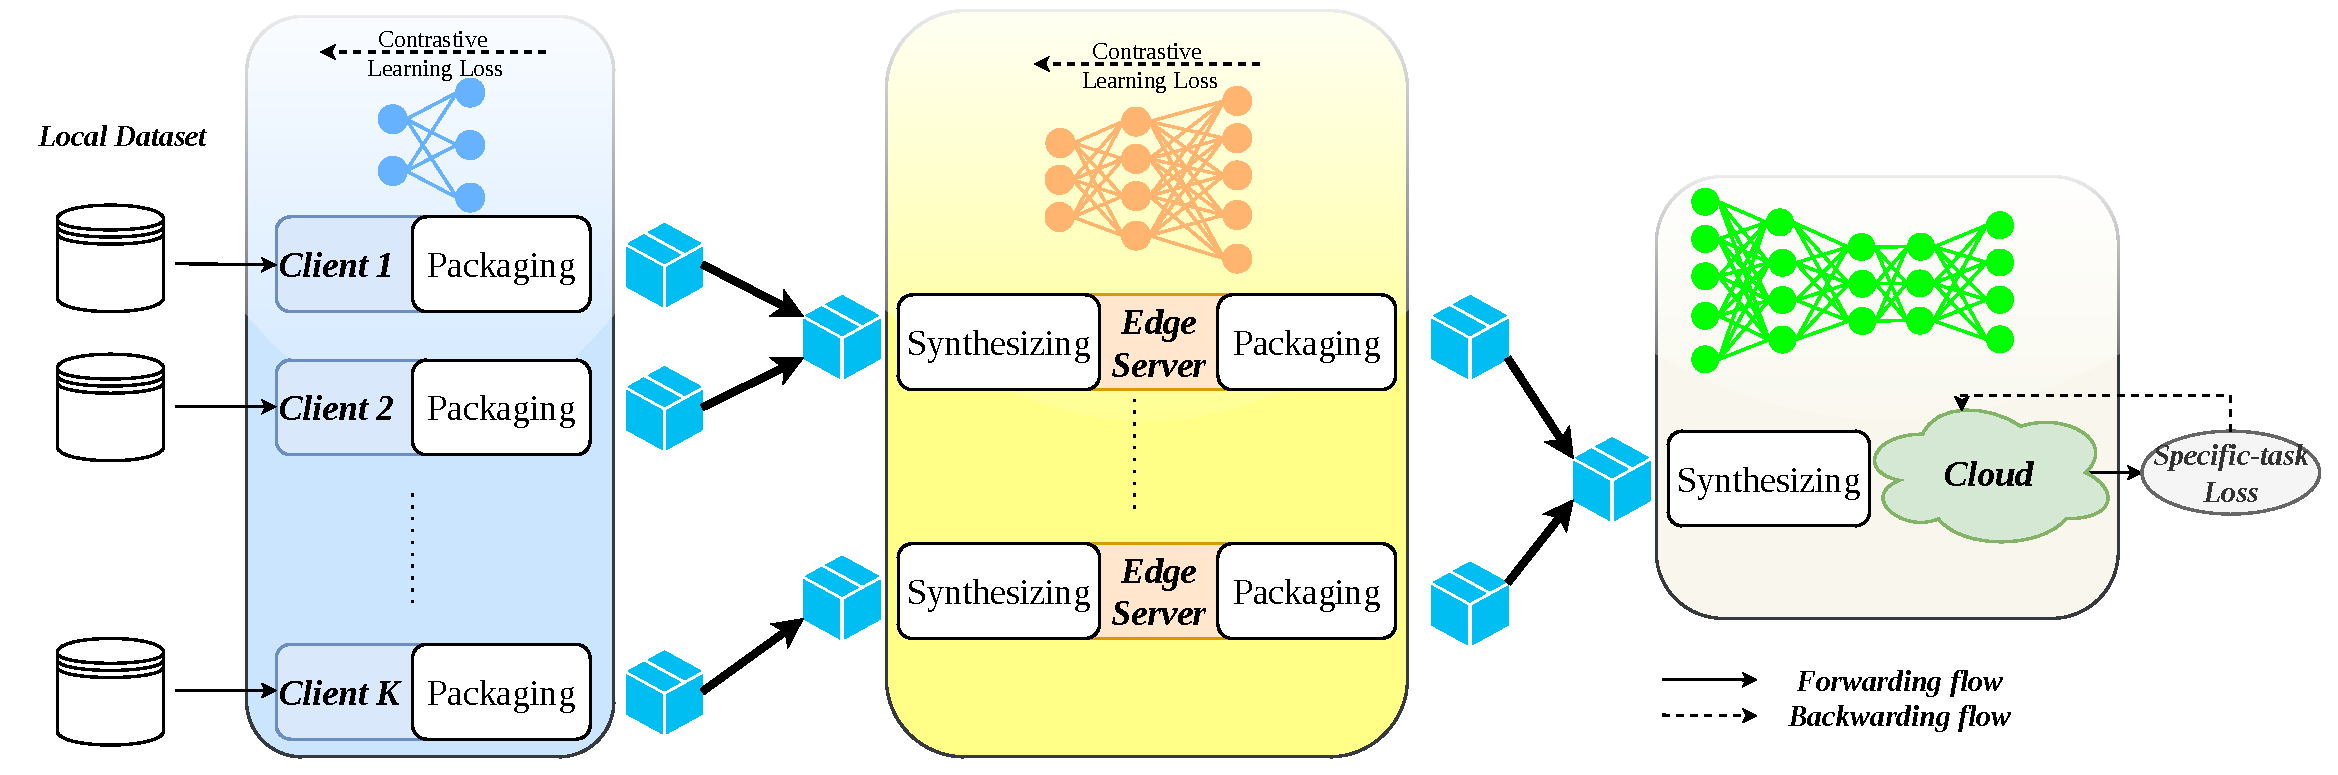
\includegraphics[width=\linewidth]{figures/method-2.pdf}
    \caption{The \hsfp hierarchy. Clients communicate class-wise prototype statistics to edge servers; edge and cloud tiers aggregate statistics, synthesize features, and train their assigned model components without cross-tier backpropagation.}
    \label{fig:hsfp_framework}
\end{figure}

The key design choice in \hsfp is to replace sample-level smashed activations and cross-tier gradients with class-wise prototype statistics. For class $j$, client $k$ computes a feature mean $\pmu_k^{(j)}$, feature standard deviation $\psigma_k^{(j)}$, and support count $n_k^{(j)}$ from its local representation space. The transmitted packet is therefore
\begin{equation}
    P_k^{(j)}=\left(\pmu_k^{(j)},\psigma_k^{(j)},n_k^{(j)}\right),
\end{equation}
rather than a batch of per-sample activations. Edge server $\edgeidx$ aggregates packets from $k\in\clients_{\edgeidx}$ into edge-level class-wise prototype statistics, and the cloud similarly aggregates edge statistics into global class-wise prototype statistics.

Upper tiers then synthesize features from the received statistics. For an aggregated class statistic $(\pmu^{(j)},\psigma^{(j)})$, a synthetic feature is sampled as
\begin{equation}
    z^{(j)} = \pmu^{(j)} + \psigma^{(j)} \odot \epsilon,\qquad
    \epsilon\sim\mathcal{N}(0,I),
    \label{eq:prelim_synthesis}
\end{equation}
which corresponds to a diagonal Gaussian approximation of the lower-tier feature distribution. This Gaussian feature-synthesis strategy follows prior work on prototype-based feature augmentation and exemplar condensation for representation-preserving replay~\cite{9578909,Nguyen_2026_CVPR}. Edge models can train on synthetic client features, and the cloud model can train on synthetic edge features. The lower and upper tiers are therefore optimized through local objectives over their own inputs rather than through one end-to-end backpropagation graph.

\hsfp uses contrastive representation learning at lower tiers, following the NT-Xent contrastive objective ~\cite{chen2020simple}, so that class-wise prototype statistics preserve discriminative structure. The practical benefit is communication reduction: clients send $O(J_k d)$ statistics for $J_k$ observed classes and feature dimension $d$, rather than transmitting activations and gradients for every sample and every split-learning iteration. The methodological limitation, which motivates \ehsfp, is that the original framework assumes comparatively stable prototype availability. It does not explicitly model stateless learning episodes, stale prototype updates, partial prototype updates, missing prototype packets, or asynchronous edge/cloud aggregation.

\section{Problem Formulation}
\label{sec:formulation}

We formulate \ehsfp as hierarchical split-federated optimization over time-varying prototype-induced feature distributions. The client set is $\clients=\bigcup_{\edgeidx=1}^{M}\clients_{\edgeidx}$, where $\clients_{\edgeidx}$ denotes the clients associated with edge server $\edgeidx$. Client $k$ has local data $\mathcal{D}_k=\{(x_i,y_i)\}$ and produces, for class $j$, a prototype packet $P_{k,t}^{(j)}=(\pmu_{k,t}^{(j)},\psigma_{k,t}^{(j)},n_{k,t}^{(j)})$ at round or event index $t$.

\begin{definition}[Episodic prototype learning]
A stateless learning episode is an invocation of an edge or cloud learner that starts from the current available model state and receives a subset of prototype packets rather than a guaranteed complete synchronized round. Let $\mathcal{E}_t$ denote the episode at index $t$, and let $\mathcal{P}_t$ be the packets available to that episode. Episodic prototype learning optimizes upper-tier models using the synthetic distribution induced by $\mathcal{P}_t$ and, optionally, by an episodic prototype memory $\mem_t$.
\end{definition}

\begin{definition}[Partial prototype updates]
At episode $t$, only a participating subset $\clients_t\subseteq\clients$ contributes packets. The participation rate is $\rho_t=|\clients_t|/|\clients|$. For edge $\edgeidx$, the local participating set is $\clients_{\edgeidx,t}=\clients_t\cap\clients_{\edgeidx}$. Partial prototype updates occur whenever $\rho_t<1$ or when only a subset of classes is represented among participating clients.
\end{definition}

\begin{definition}[Stale prototype updates]
A packet from client $k$ used in episode $t$ may have been generated at an earlier episode index $s\leq t$. Its staleness is $\stale_{k,t}=t-s$, with $\stale_{k,t}\leq \stale_{\max}$. Stale prototype updates therefore train upper tiers using $(\pmu_{k,s}^{(j)},\psigma_{k,s}^{(j)},n_{k,s}^{(j)})$ while the current reference client distribution may be indexed by $t$.
\end{definition}

\begin{definition}[Missing prototype packets]
For each expected packet, let $B_{k,t}^{(j)}\sim\mathrm{Bernoulli}(1-\dropoutp)$ indicate whether the packet is available to episode $t$. A missing prototype packet occurs when $B_{k,t}^{(j)}=0$. This models missing events, timeouts, and partial execution in event-driven or serverless-style deployments, but the contribution remains the learning formulation rather than the deployment substrate.
\end{definition}

\begin{definition}[Asynchronous edge/cloud aggregation]
Each edge server aggregates available client packets whenever its local episode is triggered. The cloud aggregates edge-level packets every $H$ edge rounds or when an event-driven trigger condition is satisfied. Thus, edge updates and cloud updates need not share a single synchronized clock.
\end{definition}

Given available packets and memory, an upper tier constructs class-wise synthetic distributions
\begin{equation}
    Q_{t}^{(j)}=\mathcal{N}\left(\widehat{\pmu}_{t}^{(j)},
    \mathrm{diag}\left((\widehat{\psigma}_{t}^{(j)})^2\right)\right),
\end{equation}
where $\widehat{\pmu}_{t}^{(j)}$ and $\widehat{\psigma}_{t}^{(j)}$ are aggregated from partial, stale, and memory-replayed prototype statistics. Let $Q_{*,t}^{(j)}$ denote the current reference feature distribution that would be induced by complete, fresh class-wise statistics at episode $t$.

\begin{definition}[Prototype-induced distributional drift]\label{def:proto_drift}
For class $j$, the prototype-induced distributional drift is the squared 2-Wasserstein distance between the synthesized distribution used by an upper tier and the current reference feature distribution:
\begin{equation}
    \drift_t^{(j)}
    = W_2^2\left(Q_t^{(j)},Q_{*,t}^{(j)}\right).
\end{equation}
Under diagonal Gaussian prototype models, if $Q_t^{(j)}=\mathcal{N}(\widehat{\pmu}_t^{(j)},\mathrm{diag}((\widehat{\psigma}_t^{(j)})^2))$ and $Q_{*,t}^{(j)}=\mathcal{N}(\pmu_{*,t}^{(j)},\mathrm{diag}((\psigma_{*,t}^{(j)})^2))$, then
\begin{equation}
    \drift_t^{(j)}
    = \left\|\widehat{\pmu}_t^{(j)}-\pmu_{*,t}^{(j)}\right\|_2^2
    + \left\|\widehat{\psigma}_t^{(j)}-\psigma_{*,t}^{(j)}\right\|_2^2.
\end{equation}
The aggregate drift is $\drift_t=\sum_{j=1}^{J}\pi_t^{(j)}\drift_t^{(j)}$, where $\pi_t^{(j)}$ is a class weight such as the normalized support count.
\end{definition}

Let $W_c$, $W_e$, and $W_g$ denote client, edge, and cloud model components. The ideal hierarchical empirical risk is
\begin{equation}
    \begin{split}
    &\min_{W_c,W_e,W_g}
    F(W_c,W_e,W_g)
    \\
    &\;\;=
    \sum_{k\in\clients}\frac{|\mathcal{D}_k|}{|\mathcal{D}|}\,
    \mathbb{E}_{(x,y)\sim\mathcal{D}_k}
    \bigl[\ell\bigl(W_g\circ W_e\circ W_c(x),y\bigr)\bigr].
    \end{split}
    \label{eq:global_objective}
\end{equation}
\ehsfp minimizes this objective under the constraints that upper-tier gradients are computed from $Q_t^{(j)}$ rather than raw lower-tier activations, packet availability is partial and random, packet ages satisfy $\stale_{k,t}\leq\stale_{\max}$, and edge/cloud aggregation is asynchronous. The analysis in later sections will bound the resulting stationarity gap in terms of stochastic optimization error, aggregation interval error, stale prototype updates, partial prototype updates, memory replay error, and the aggregate drift $\drift_t$.

\section{The E-HSFP Framework}
\label{sec:method}

\subsection{Overview}
\ehsfp extends \hsfp by treating each upper-tier invocation as a stateless learning episode that may receive incomplete, stale, or partial prototype packets. The framework keeps the class-wise prototype statistics interface from \hsfp, namely $(\pmu_{k,t}^{(j)},\psigma_{k,t}^{(j)},n_{k,t}^{(j)})$, but augments the edge and cloud learners with five stability-oriented modules. Episodic prototype memory bounds the error induced by missing-update replacement; reliability-aware prototype aggregation reduces variance and stale prototype updates by down-weighting unreliable packets; prototype replay consistency controls the prototype-induced distributional drift in Definition~\ref{def:proto_drift}; prototype dropout regularization trains upper tiers to tolerate missing packets as a learning augmentation; and the optional residual prototype generator reduces synthesis bias while preserving the original client communication payload. The resulting update path is: receive available packets, read memory, aggregate with reliability weights, synthesize current and replayed features, optimize the upper-tier objective, and write refreshed statistics back to memory.

\subsection{Episodic Prototype Memory}
For edge server $\edgeidx$ and class $j$, \ehsfp stores a bounded episodic prototype memory
\begin{equation}
    \mem_{\edgeidx,t}^{(j)}
    =
    \left\{
    \left(\pmu_{\edgeidx,t'}^{(j)},\psigma_{\edgeidx,t'}^{(j)},
    n_{\edgeidx,t'}^{(j)},a_{t'}\right)
    \right\}_{t'\leq t},
\end{equation}
where $a_{t'}=t-t'$ is an age tag and the memory is bounded by a FIFO capacity, $|\mem_{\edgeidx,t}^{(j)}|\leq \memcap$. We use $\memcap$ rather than $M$ to avoid overloading the number of edge servers in $\clients=\bigcup_{\edgeidx=1}^{M}\clients_{\edgeidx}$. The memory induces a replay distribution $Q_{\mathrm{memory},\edgeidx,t}^{(j)}$ from the stored statistics, while the packets available to the current stateless learning episode induce $Q_{\mathrm{current},\edgeidx,t}^{(j)}$. The edge learner trains on the mixture
\begin{equation}
    % \begin{split}
    Q_{\edgeidx,t}^{(j)}
    =
    \alpha_t Q_{\mathrm{current},\edgeidx,t}^{(j)}
    +
    (1-\alpha_t)Q_{\mathrm{memory},\edgeidx,t}^{(j)},
    % \end{split}
    \label{eq:memory_mixture}
\end{equation}
\begin{equation*}
    \begin{split}
    \alpha_t
    &=
    \min\left\{
    1,
    \right.
    \\
    &\quad
    \left.
    \frac{N_{\mathrm{cur},\edgeidx,t}^{(j)}}
    {N_{\mathrm{cur},\edgeidx,t}^{(j)}
    +N_{\mathrm{mem},\edgeidx,t}^{(j)}
    +\varepsilon}
    \right\}.
    \end{split}
\end{equation*}
where $N_{\mathrm{cur},\edgeidx,t}^{(j)}$ and $N_{\mathrm{mem},\edgeidx,t}^{(j)}$ denote current and memory support totals and $\varepsilon>0$ prevents division by zero. When packets are missing or stale, the edge or cloud samples from $Q_{\mathrm{memory},\edgeidx,t}^{(j)}$ to perform distributional replay. This bounded-memory replay design follows the exemplar-replay principle established in continual learning~\cite{rebuffi2017icarl}, adapted here to class-wise prototype statistics rather than raw exemplars so that memory cost and communication payload remain independent of the number of stored samples. Thus, each asynchronous edge/cloud aggregation call is implemented as a stateless learning episode: it reads available packets and memory, updates its upper-tier model, emits refreshed class-wise prototype statistics, and terminates without requiring a persistent per-client optimizer state.

\subsection{Reliability-Aware Prototype Aggregation}
Given current or memory-replayed packets from clients $k\in\clients_{\edgeidx}$, \ehsfp computes a reliability score for each class-wise prototype statistic. Let $a_k$ be the packet age and let $\bar{\pmu}^{(j)}$ be a robust reference mean from the available class-$j$ packets, such as a support-weighted mean from the previous episode. We use the analyzable monotone form
\begin{equation}
    \begin{split}
    w_k^{(j)}
    &=
    g_{\phi}\!\left(n_k^{(j)},\|\psigma_k^{(j)}\|,a_k,
    d(\pmu_k^{(j)},\bar{\pmu}^{(j)})\right)
    \\
    &=
    \frac{(n_k^{(j)})^{\beta}}
    {(\|\psigma_k^{(j)}\|_2^2+\epsilon_{\sigma})^{\gamma}}
    e^{-\rho a_k}
    e^{-\chi d(\pmu_k^{(j)},\bar{\pmu}^{(j)})^2},
    \end{split}
    \label{eq:reliability_weight}
\end{equation}
where $\phi=(\beta,\gamma,\rho,\chi,\epsilon_{\sigma})$ are fixed hyperparameters with nonnegative exponents and decay rates. This is a learning module for reducing the influence of noisy or stale prototype packets, not a resource-allocation mechanism. The weighting scheme is inspired by robust and trust-aware aggregation in federated learning~\cite{blanchard2017krum,cao2021fltrust}, but differs by operating on prototype-packet metadata (support count, variance, age, distributional distance) rather than robustifying raw gradient or parameter updates directly. The class-wise edge mean is
\begin{equation}
    \pmu_{\edgeidx}^{(j)}
    =
    \frac{\sum_{k\in\clients_{\edgeidx}}w_k^{(j)}\pmu_k^{(j)}}
    {\sum_{k\in\clients_{\edgeidx}}w_k^{(j)}},
    \label{eq:agg_mean}
\end{equation}
and the diagonal variance follows the law of total variance:
\begin{equation}
    (\psigma_{\edgeidx}^{(j)})^2
    =
    \frac{\sum_{k\in\clients_{\edgeidx}}w_k^{(j)}
    \left((\psigma_k^{(j)})^2+
    (\pmu_k^{(j)}-\pmu_{\edgeidx}^{(j)})^2\right)}
    {\sum_{k\in\clients_{\edgeidx}}w_k^{(j)}}.
    \label{eq:agg_var}
\end{equation}
The same equations apply at the cloud tier after replacing client packets by edge-level packets.

\subsection{Prototype Replay Consistency}
Let $h_e$ denote the edge sub-model feature map. For each class $j$, sample $z_{\mathrm{current}}^{(j)}\sim Q_{\mathrm{current},\edgeidx,t}^{(j)}$ and $z_{\mathrm{memory}}^{(j)}\sim Q_{\mathrm{memory},\edgeidx,t}^{(j)}$ using the same class label. Prototype replay consistency penalizes feature disagreement between current and replayed synthetic inputs:
\begin{equation}
    \mathcal{L}_{\mathrm{PRC}}
    =
    \sum_{j=1}^{J}
    \left\|
    h_e\!\left(z_{\mathrm{current}}^{(j)}\right)
    -
    h_e\!\left(z_{\mathrm{memory}}^{(j)}\right)
    \right\|_2^2 .
    \label{eq:prc_loss}
\end{equation}
Because $\drift_t$ measures the Wasserstein discrepancy between the synthesized distribution and the current complete-reference distribution in Definition~\ref{def:proto_drift}, this loss is used as a practical surrogate for reducing the sensitivity of upper-tier features to memory replay and stale prototype updates.

\subsection{Prototype Dropout Regularization}
During upper-tier training, we independently remove each prototype packet with probability $\dropoutp_{\mathrm{train}}$. Let $z_{\mathrm{full}}$ be synthesized from the full available packet set, and let $z_{\mathrm{drop}}$ be synthesized after applying the dropout mask. \ehsfp adds
\begin{equation}
    \mathcal{L}_{\mathrm{drop}}
    =
    D_{\mathrm{KL}}\!\left(
    p(y\mid z_{\mathrm{full}})
    \,\middle\|\,
    p(y\mid z_{\mathrm{drop}})
    \right),
    \label{eq:drop_loss}
\end{equation}
which teaches edge and cloud models to keep predictions stable under partial prototype updates. This is the single place where the serverless-style motivation enters the method: dropout simulates event timeouts and partial execution as a learning augmentation, rather than a deployment mechanism.

\subsection{Residual Prototype Generator}
The residual prototype generator is an optional upper-tier module for reducing Gaussian synthesis bias. Instead of sampling only from the diagonal prototype model in \eqref{eq:prelim_synthesis}, the upper tier can synthesize
\begin{equation}
    z_{\mathrm{syn}}
    =
    \pmu^{(j)}
    +
    \psigma^{(j)}\odot\epsilon
    +
    G_{\theta}\!\left(\pmu^{(j)},\psigma^{(j)},\epsilon\right),
    \qquad
    \epsilon\sim\mathcal{N}(0,I).
    \label{eq:residual_synthesis}
\end{equation}
The lightweight residual $G_{\theta}$ is trained only at the edge or cloud tier using synthetic replay objectives. Clients still transmit only $(\pmu_k^{(j)},\psigma_k^{(j)},n_k^{(j)})$, so the communication cost of class-wise prototype statistics is unchanged.

\subsection{Per-Edge Objective and Algorithm}
For the edge server $\edgeidx$, the training loss combines the inherited \hsfp contrastive/classification loss with the two episodic stabilizers:
\begin{equation}
    \mathcal{L}_{e}
    =
    \mathcal{L}_{\mathrm{con}}
    +
    \lambda_{\mathrm{prc}}\mathcal{L}_{\mathrm{PRC}}
    +
    \lambda_{\mathrm{drop}}\mathcal{L}_{\mathrm{drop}} .
    \label{eq:edge_loss}
\end{equation}
Here $\mathcal{L}_{\mathrm{con}}$ is the contrastive/classification objective inherited from \hsfp as summarized in Section~\ref{sec:preliminary}. The cloud uses the same episodic aggregation, memory, dropout, and replay-consistency mechanisms with its supervised classifier loss in place of the edge contrastive loss.

\begin{algorithm}[t]
\caption{E-HSFP Episodic Edge/Cloud Update}
\label{alg:ehsfp}
\begin{algorithmic}[1]
\Require Episode index $t$, edge $\edgeidx$, available packets $\mathcal{P}_{\edgeidx,t}$, memories $\{\mem_{\edgeidx,t-1}^{(j)}\}_{j=1}^{J}$, upper-tier model $h_e$, dropout probability $\dropoutp_{\mathrm{train}}$
\Ensure Updated upper-tier model and refreshed class-wise prototype statistics
\For{each class $j$ observed in $\mathcal{P}_{\edgeidx,t}$ or $\mem_{\edgeidx,t-1}^{(j)}$}
    \State Read current packets $\{(\pmu_{k,t}^{(j)},\psigma_{k,t}^{(j)},n_{k,t}^{(j)})\}$ and memory entries $\mem_{\edgeidx,t-1}^{(j)}$
    \State Assign ages $a_k$ to current, stale, and replayed packets
    \State Compute reliability weights $w_k^{(j)}$ using \eqref{eq:reliability_weight}
    \State Aggregate $\pmu_{\edgeidx,t}^{(j)}$ and $\psigma_{\edgeidx,t}^{(j)}$ using \eqref{eq:agg_mean}--\eqref{eq:agg_var}
    \State Construct $Q_{\edgeidx,t}^{(j)}$ from the current-memory mixture in \eqref{eq:memory_mixture}
    \State Sample $z_{\mathrm{current}}^{(j)}$, $z_{\mathrm{memory}}^{(j)}$, $z_{\mathrm{full}}^{(j)}$, and $z_{\mathrm{drop}}^{(j)}$
\EndFor
\State Compute $\mathcal{L}_{\mathrm{PRC}}$ by \eqref{eq:prc_loss} and $\mathcal{L}_{\mathrm{drop}}$ by \eqref{eq:drop_loss}
\State Update $h_e$ using $\nabla\mathcal{L}_e$ from \eqref{eq:edge_loss}
\State Compute refreshed output statistics $(\pmu_{\edgeidx,t}^{(j)},\psigma_{\edgeidx,t}^{(j)},n_{\edgeidx,t}^{(j)})$ for each class $j$
\State Write refreshed statistics to $\mem_{\edgeidx,t}^{(j)}$ with age tag $a_t=0$ and evict FIFO entries beyond capacity $\memcap$
\State Send edge-level packets to the cloud when the asynchronous trigger fires; the cloud repeats the same episodic update over edge-level packets
\end{algorithmic}
\end{algorithm}

\section{Convergence Analysis}
\label{sec:convergence}

This section analyzes \ehsfp as a perturbation of tier-wise non-convex stochastic optimization under synthesized prototype distributions. The goal is not to claim convergence to a global optimum, but to bound convergence to a stationary neighborhood whose radius depends on stochastic gradients, hierarchical aggregation, prototype variance, stale prototype updates, partial prototype updates, missing prototype packets, and prototype-induced distributional drift.

\begin{assumption}[Smooth tier objectives]\label{asm:smooth}
The ideal objective $F$ in \eqref{eq:global_objective} and each tier objective induced by edge or cloud synthetic distributions are $L$-smooth in their trainable parameters.
\end{assumption}

\begin{assumption}[Stochastic gradients]\label{asm:variance}
For the current synthetic distribution used in episode $t$, the stochastic gradient $g_t$ is conditionally unbiased for the corresponding tier objective and satisfies $\mathbb{E}[\|g_t-\nabla F_t(\theta_t)\|_2^2\mid\mathcal{F}_t]\leq\sigma_g^2$.
\end{assumption}

\begin{assumption}[Bounded prototype variance]\label{asm:proto_var}
For all clients $k$, edges $\edgeidx$, classes $j$, and episodes $t$, $\|\psigma_{k,t}^{(j)}\|_2^2\leq S_{\max}^2$ and $\|\pmu_{k,t}^{(j)}\|_2\leq B_{\mu}$. The same bounds hold for edge-level aggregated prototype statistics.
\end{assumption}

\begin{assumption}[Bounded staleness]\label{asm:staleness}
Any packet used in episode $t$ has staleness $\stale_{k,t}\leq\stale_{\max}$, and any replayed memory entry has age at most $A_{\mem}$ after FIFO eviction.
\end{assumption}

\begin{assumption}[Bounded prototype-induced drift]\label{asm:drift}
The aggregate drift from Definition~\ref{def:proto_drift} satisfies $\mathbb{E}[\drift_t]\leq D_{\max}$ for all $t$. In addition, the loss gradient is $L_z$-Lipschitz with respect to synthetic feature inputs in Wasserstein distance.
\end{assumption}

\begin{assumption}[Partial participation]\label{asm:participation}
Each expected class-wise packet is observed with probability at least $q_{\min}>0$, and missing events follow the Bernoulli model in Section~\ref{sec:formulation} with drop probability $\dropoutp<1$.
\end{assumption}

\begin{assumption}[Bounded heterogeneity and hierarchical aggregation error]\label{asm:het_agg}
There exist constants $H_{\mathrm{client}}\geq0$ and $H_{\mathrm{agg}}\geq0$ such that the expected squared dissimilarity between client-level gradients and the corresponding edge-level objective gradient is at most $H_{\mathrm{client}}$ (bounded client drift under statistical heterogeneity), and the expected squared perturbation introduced by one asynchronous edge/cloud aggregation round of the tier-wise decoupled update is at most $H_{\mathrm{agg}}$.
\end{assumption}

\begin{lemma}[Prototype synthesis bias]\label{lem:synthesis_bias}
Let $\nabla F_{*,t}(\theta)$ denote the gradient under the current complete-reference feature distribution $Q_{*,t}^{(j)}$, and let $\nabla F_t(\theta)$ denote the gradient under the synthesized distribution $Q_t^{(j)}$. Under Assumptions~\ref{asm:smooth} and~\ref{asm:drift},
\begin{equation}
    \begin{split}
    \left\|
    \nabla F_t(\theta)-\nabla F_{*,t}(\theta)
    \right\|_2
    &\leq
    L_z
    \left(\sum_{j=1}^{J}\pi_t^{(j)}\drift_t^{(j)}\right)^{1/2}
    \\
    &=
    L_z\sqrt{\drift_t}.
    \end{split}
\end{equation}
\end{lemma}
\begin{proof}
For diagonal Gaussian prototype models, Definition~\ref{def:proto_drift} gives the squared 2-Wasserstein discrepancy as the sum of squared mean and standard-deviation errors. The Wasserstein Lipschitz condition in Assumption~\ref{asm:drift} then transfers this distributional discrepancy to gradient bias.
\end{proof}

\begin{lemma}[Stale prototype error]\label{lem:stale_drift}
Suppose class-wise prototype means and standard deviations move by at most $\delta_{\mu}$ and $\delta_{\sigma}$ per episode. Under Assumption~\ref{asm:staleness}, the additional gradient bias from using $\stale_{\max}$-stale prototype statistics is bounded by
\begin{equation}
    \mathbb{E}\left[
    \left\|
    \nabla F_t^{\mathrm{stale}}(\theta)
    -
    \nabla F_t^{\mathrm{fresh}}(\theta)
    \right\|_2
    \right]
    \leq
    L_z \stale_{\max}(\delta_{\mu}+\delta_{\sigma}).
\end{equation}
\end{lemma}
\begin{proof}
Unrolling the per-episode prototype displacement for at most $\stale_{\max}$ episodes gives mean and standard-deviation deviations no larger than $\stale_{\max}\delta_{\mu}$ and $\stale_{\max}\delta_{\sigma}$. Applying the same Wasserstein-to-gradient Lipschitz step as Lemma~\ref{lem:synthesis_bias} gives the stated bound.
\end{proof}

\begin{lemma}[Missing prototype packets]\label{lem:missing_update}
Let packets be independently dropped with probability $\dropoutp$. Without memory replay, inverse-probability aggregation has variance inflated by at most $(1-\dropoutp)^{-1}$ relative to complete participation. With episodic prototype memory \eqref{eq:memory_mixture}, the missing-packet contribution can be decomposed into a retained stochastic variance term and a bounded stale-replay term:
\begin{equation}
    \mathbb{E}\|\widehat{G}_{t}^{\mathrm{mem}}-G_t\|_2^2
    \leq
    \frac{C_{\mathrm{part}}\sigma_g^2}{|\clients_{\edgeidx}|(1-\dropoutp)}
    +
    C_{\mathrm{mem}}A_{\mem}^2(\delta_{\mu}+\delta_{\sigma})^2 .
\end{equation}
\end{lemma}
\begin{proof}
Bernoulli thinning gives the usual sampling-variance inflation for the observed packets. Replacing a missing packet by its memory copy avoids an unbounded missing contribution, but converts the error into a stale prototype update controlled by the memory age bound $A_{\mem}$.
\end{proof}

\begin{lemma}[Reliability-aware aggregation]\label{lem:reliability}
For a scalar coordinate of a class-wise prototype mean, suppose packet $k$ has zero-mean error variance $v_k$ and stale bias magnitude bounded by $b_k$. The inverse-error special case $w_k\propto(v_k+b_k^2)^{-1}$ minimizes the upper bound $\sum_k \alpha_k^2(v_k+b_k^2)$ over normalized linear estimators $\sum_k\alpha_k\pmu_k^{(j)}$. Consequently, this weighted estimator is no worse than uniform averaging for that bound, and it is strictly better whenever the error levels are not all equal.
\end{lemma}
\begin{proof}
The normalized linear estimator has mean-squared error upper bound $\sum_k\alpha_k^2 e_k$ with $e_k=v_k+b_k^2$. Minimizing this convex expression subject to $\sum_k\alpha_k=1$ gives $\alpha_k\propto e_k^{-1}$ by the Lagrange multiplier condition. The monotone form in \eqref{eq:reliability_weight} approximates this inverse-error behavior by increasing with support and decreasing with variance, age, and distance from the reference mean.
\end{proof}

\begin{theorem}[Stationary-neighborhood convergence]\label{thm:convergence}
Under Assumptions~\ref{asm:smooth}--\ref{asm:het_agg}, let \ehsfp run for $T$ episodes with step size $\eta=\Theta(T^{-1/2})$. For the tier-wise decoupled updates, the averaged stationarity gap satisfies
\begin{equation}
    \begin{split}
    \frac{1}{T}\sum_{t=0}^{T-1}
    \mathbb{E}\|\nabla F(\theta_t)\|_2^2
    &\leq
    \mathcal{O}\!\left(\frac{1}{\sqrt{T}}\right)
    +
    C_g\sigma_g^2
    \\
    &\quad
    +
    C_{\mathrm{het}}H_{\mathrm{client}}
    +
    C_{\mathrm{hier}}H_{\mathrm{agg}}
    \\
    &\quad
    +
    C_{\mathrm{proto}}S_{\max}^2
    +
    C_{\stale}\stale_{\max}^2
    \\
    &\quad
    +
    C_{\mathrm{miss}}\dropoutp
    +
    C_{\drift}\frac{1}{T}\sum_{t=0}^{T-1}\mathbb{E}[\drift_t].
    \end{split}
\end{equation}
Thus, \ehsfp converges to a stationary neighborhood whose radius is controlled by stochastic variance, client drift and heterogeneity, hierarchical aggregation error, prototype variance, stale prototype updates, missing prototype packets, and prototype-induced distributional drift.
\end{theorem}
\begin{proof}
Apply the descent lemma to the ideal objective evaluated at the perturbed stochastic gradient used by the current edge or cloud episode. The perturbation decomposes into stochastic gradient noise, hierarchical aggregation error inherited from tier-wise decoupling, synthesis bias from Lemma~\ref{lem:synthesis_bias}, stale prototype error from Lemma~\ref{lem:stale_drift}, missing-update error from Lemma~\ref{lem:missing_update}, and reliability-weighted aggregation error from Lemma~\ref{lem:reliability}. Summing the descent inequality over $T$ episodes and choosing $\eta=\Theta(T^{-1/2})$ yields the displayed $\mathcal{O}(1/\sqrt{T})$ term plus residual neighborhood terms.
\end{proof}

\begin{corollary}[Small episodic perturbations]\label{cor:small_perturb}
If $\stale_{\max}\rightarrow0$, $\dropoutp\rightarrow0$, and $\frac{1}{T}\sum_{t=0}^{T-1}\mathbb{E}[\drift_t]$ is controlled by the synchronous \hsfp synthetic-distribution error, then Theorem~\ref{thm:convergence} recovers a synchronous \hsfp-style $\mathcal{O}(1/\sqrt{T})$ stationarity rate with a residual neighborhood that excludes the stale-update and missing-update terms.
\end{corollary}
\begin{proof}
Set the stale prototype and Bernoulli missing-packet terms in Theorem~\ref{thm:convergence} to zero and retain the standard stochastic, heterogeneity, aggregation, and prototype-synthesis residuals.
\end{proof}

The bound explains the role of each \ehsfp module. Episodic prototype memory shrinks the missing-update term by replacing absent packets with bounded-age replay. Reliability-aware prototype aggregation reduces the variance and staleness constants by assigning smaller weights to uncertain, old, or outlying packets. Prototype replay consistency reduces the sensitivity to $\drift_t$ by aligning current and memory-induced features. Prototype dropout regularization reduces the sensitivity constant of the missing-update term by training on packet masks. The optional residual prototype generator reduces the synthesis-bias constant by improving the match between diagonal Gaussian prototypes and upper-tier synthetic features.

% Table rows are generated from recorded runs by Sources/scripts/journal_experiments/fill_manuscript.py.
% \tabrows uses the TeX primitive input so it works inside tabular.
% \figorph{file}{text}: include the generated figure if it exists, else keep the placeholder box.
\providecommand{\figorph}[2]{\IfFileExists{#1}{\includegraphics[width=\linewidth]{#1}}{\fbox{\parbox[c][5cm][c]{0.9\linewidth}{\centering #2}}}}
\makeatletter\providecommand{\tabrows}[1]{\@@input #1 }\makeatother
\InputIfFileExists{generated/prose_values}{}{}
\section{Experimental Evaluation}
\label{sec:experiments}

\subsection{Experimental Setup}
The experimental campaign evaluates \ehsfp under hierarchical split-federated learning with complete, partial, stale, and episodic prototype arrivals. Journal-protocol classification experiments use CIFAR-10 and CIFAR-100~\cite{krizhevsky2009learning} and HAM10000~\cite{tschandl2018ham10000}; ImageNet-1K~\cite{5206848} appears only in the conference-reference tables, because no journal-protocol ImageNet-1K runs were performed. Segmentation experiments use ISIC-2018, following the skin-lesion challenge protocol lineage in~\cite{8363547}. The compared methods are FedAvg~\cite{mcmahan2017communication}, FedProx~\cite{li2020federated}, FedNova~\cite{10.5555/3495724.3496362}, HierFL~\cite{liu2020client,9488756}, SplitFed~\cite{thapa2022splitfed}, HeteroSFL, HSFL~\cite{quan2023hiersfl}, the conference \hsfp baseline summarized in Section~\ref{sec:preliminary}, and \ehsfp.

Data are partitioned into IID, mildly non-IID, and severely non-IID client splits. Non-IID splits use class-proportion Dirichlet sampling with concentration $0.7$ (mild) and $0.3$ (severe), fixed random seeds, and identical client counts across compared methods. % TODO(result): Confirm the exact Dirichlet concentration values for mild and severe non-IID partitions after the simulation configuration is frozen.
The episodic stress protocol varies prototype dropout rate $\dropoutp$, staleness bound $\stale$, asynchronous edge/cloud aggregation interval, and serverless-style event loss, timeout, and cold-start conditions. These stressors are included to test whether stateless learning episodes can remain stable when prototype packets arrive incompletely or late.

Evaluation metrics include accuracy, macro F1-score, communication volume, client memory, edge memory, cloud memory, rounds to convergence, training time, Dice, IoU, prototype drift, and stability. Prototype drift follows Definition~\ref{def:proto_drift}. For a validation-accuracy sequence $\{a_t\}$ and a trailing window $\mathcal{W}_t$, the stability metric is defined as
\begin{equation}
    \mathrm{Stability}(t)
    =
    \frac{1}{|\mathcal{W}_t|}
    \sum_{s\in\mathcal{W}_t}
    \left(a_s-\frac{1}{|\mathcal{W}_t|}\sum_{r\in\mathcal{W}_t}a_r\right)^2 .
\end{equation}
Lower values indicate smaller validation oscillation over the trailing window. We use $|\mathcal{W}_t|=5$ and report the value at the final round in units of $\%^2$. Rounds to convergence is the first round at which the three-round moving average of validation accuracy reaches 95\% of the best accuracy observed in the run and remains there for three rounds. Prototype drift is the edge-tier squared 2-Wasserstein drift of Definition~\ref{def:proto_drift}, averaged over edges and rounds. Communication is the total traffic over the run in GB.

\paragraph{Implementation.}
All journal-protocol classification runs use 200 clients grouped under 5 edge servers, 10\% client participation per round, 60 communication rounds, a local batch size of 16, and Adam with learning rate $10^{-4}$, weight decay $10^{-4}$, and a five-round warm-up followed by a learning-rate schedule. On CIFAR-100, the client holds an 11.2M-parameter ResNet-18 trunk, the edge holds a 0.69M-parameter module, and the cloud holds a linear classifier. The full \ehsfp configuration uses episodic prototype memory (capacity 500, replay ratio 0.3, maximum prototype age 20), prototype dropout with rate 0.2, reliability-aware aggregation, replay consistency, and low-rank shared-covariance synthesis. It also runs with simulated serverless events: cold starts with probability 0.15 and function timeouts with probability 0.05. The \hsfp rows use the same backbone, partitions, and schedule but no simulated events. Consequently, \hsfp--\ehsfp accuracy comparisons are conservative for \ehsfp, while their prototype-drift values are not directly comparable. % TODO(result): Confirm hardware and the edge/cloud intervals before submission.

\paragraph{Protocol separation and result provenance.}
We keep three result streams strictly disjoint. First, the \emph{conference-reference protocol} contains the five-run results reported in the accepted ECCV 2026 paper, including 200 distributed devices and the aggregation intervals stated in each table caption. Second, the \emph{proxy protocol} uses 10 communication rounds and three date-based seeds (20260714--20260716); it is used only for implementation diagnosis and is not used for paper-level comparisons. Third, the \emph{frozen journal protocol} uses 60 rounds and integer seeds. The matched method comparisons (Tables~\ref{tab:journal_main_classification} and~\ref{tab:journal_segmentation}) use five seeds, $\{0,1,2,3,4\}$. The robustness, ablation, and scalability sweeps use a single run with seed 0 per cell. The convergence curves in Figure~\ref{fig:conv_curves} use seeds $\{0,1,2\}$. Single-seed differences smaller than the five-seed standard deviations of Table~\ref{tab:journal_main_classification} (0.3--0.6 points on CIFAR) should therefore not be read as effects. Consequently, proxy, legacy 60-round, and conference-reference values are never pooled, rescaled, or compared as if they were generated by a common protocol. Unless otherwise stated, reported uncertainty is the sample standard deviation over independent runs.

% INTERNAL STATUS (2026-07-22): no completed Full E-HSFP result is available.
% The hsfp_memory_reliability_prc and full_e_hsfp presets are blocked by an
% unresolved autograd deadlock. Keep E-HSFP cells as \pending until genuine,
% traceable five-seed results exist under the frozen journal protocol.

\subsection{Convergence Behavior}
This subsection connects the empirical campaign to Theorem~\ref{thm:convergence} and Corollary~\ref{cor:small_perturb}. Figure~\ref{fig:conv_curves} shows validation curves under IID and non-IID partitions (mean over seeds $\{0,1,2\}$). At round 60, \ehsfp is ahead of \hsfp on CIFAR-10 IID (49.25 vs.\ 45.61\%) and $dir(0.7)$ (39.70 vs.\ 36.61\%). Under $dir(0.3)$ the two are indistinguishable (35.30$\pm$3.24 vs.\ 35.22$\pm$0.14\%), with a much larger seed-to-seed spread for \ehsfp. On CIFAR-100 IID, \ehsfp leads 48.24 vs.\ 44.96\%. On HAM10000, \ehsfp reaches 67.27--70.66\% across the three partitions, whereas \hsfp stays at 40.44--54.40\% with standard deviations of up to 7.6 points. The seed-0 \hsfp runs on HAM10000 never meet the convergence rule above (Table~\ref{tab:noniid_robustness}). Figure~\ref{fig:drift_rounds} shows prototype drift over rounds under the episodic stress protocol. The stability-bound term of Figure~\ref{fig:bound_vs_drift} has not been evaluated numerically, because the constants of Theorem~\ref{thm:convergence} have not been instantiated for these models; the corresponding column of Table~\ref{tab:staleness_convergence} is marked n/a.

% TODO(figure): Replace placeholder with final plot after simulations are completed.
\begin{figure}[t]
    \centering
    \figorph{figures/fig_conv_curves.pdf}{Placeholder: convergence curves under IID and non-IID partitions (final plot pending simulations)}
    \caption{Validation convergence curves for IID and non-IID classification protocols.}
    \label{fig:conv_curves}
\end{figure}

% TODO(figure): Replace placeholder with final plot after simulations are completed.
\begin{figure}[t]
    \centering
    \figorph{figures/fig_drift_rounds.pdf}{Placeholder: prototype drift over communication rounds (final plot pending simulations)}
    \caption{Prototype-induced distributional drift over rounds under the episodic stress protocol.}
    \label{fig:drift_rounds}
\end{figure}

% TODO(figure): Replace placeholder with final plot after simulations are completed.
\begin{figure}[t]
    \centering
    \fbox{\parbox[c][5cm][c]{0.9\linewidth}{\centering Placeholder: stability-bound term versus empirical drift (final plot pending simulations)}}
    \caption{Comparison between the stability-bound term from the convergence analysis and empirical prototype drift.}
    \label{fig:bound_vs_drift}
\end{figure}

\subsection{Main Results}
Tables~\ref{tab:main_classification} and~\ref{tab:segmentation} reproduce the accepted conference-reference results verbatim; they establish the H-SFP baseline that the journal extension must compare against. These values are not pooled with the proxy or legacy 60-round diagnostics. Under the matched conference protocol, H-SFP provides the highest federated accuracy on all four classification datasets. It exceeds the strongest reported federated baseline by 3.99 percentage points on CIFAR-10, 2.00 points on CIFAR-100, 7.76 points on HAM10000, and 1.1 points on ImageNet-1K.

Table~\ref{tab:journal_main_classification} repeats the comparison under the frozen journal protocol with five seeds. \ehsfp improves on \hsfp on every dataset: by 3.71 points on CIFAR-10 (49.14$\pm$0.27 vs.\ 45.43$\pm$0.27), 3.19 points on CIFAR-100 (48.05$\pm$0.59 vs.\ 44.86$\pm$0.30), and 25.80 points on HAM10000 (67.21$\pm$1.15 vs.\ 41.41$\pm$2.74). This improvement holds even though the \ehsfp runs include simulated serverless events. However, the conference ranking is not reproduced under this protocol. Both prototype-based methods trail the strongest weight-sharing baselines: HSFL (A) reaches 73.75\% on CIFAR-10 and 58.24\% on CIFAR-100, and SplitFed reaches 78.31\% on HAM10000. FedAvg, FedProx, HierFL, and SplitFed also exceed \ehsfp on all three datasets. \ehsfp is ahead only of FedNova and HeteroSFL, both of which degrade severely under this protocol. The journal-protocol \hsfp is also far below its conference-reference accuracy (45.43 vs.\ 67.44\% on CIFAR-10), which suggests that the gap originates in the shared prototype pipeline under this backbone and budget rather than in the E-HSFP modules. The present evidence therefore supports \ehsfp as an improvement over \hsfp under episodic stress, but not as a state-of-the-art federated classifier.

\begin{table*}[t]
\centering
\caption{Conference-reference classification accuracy (\%) across 200 distributed devices. CIFAR-10 and CIFAR-100 use IID partitions; HAM10000 and ImageNet-1K use ResNet-50 under IID partitions. HSFL and H-SFP use aggregation interval (A), $I_c=5$ and $I_e=10$. Results are mean $\pm$ standard deviation over five independent runs and are reproduced verbatim from the accepted ECCV 2026 paper. E-HSFP remains pending under the frozen journal protocol.}
\label{tab:main_classification}
\begin{tabular}{@{}lcccc@{}}
\toprule
Method & CIFAR-10 & CIFAR-100 & HAM10000 & ImageNet-1K \\
\midrule
FedAvg    & 57.25 {\scriptsize $\pm$ 1.24} & 48.85 {\scriptsize $\pm$ 1.40} & 68.28 {\scriptsize $\pm$ 1.45} & 23.1 {\scriptsize $\pm$ 1.4} \\
FedProx   & 58.25 {\scriptsize $\pm$ 1.20} & 52.75 {\scriptsize $\pm$ 1.25} & 71.15 {\scriptsize $\pm$ 1.30} & 24.1 {\scriptsize $\pm$ 1.3} \\
FedNova   & 23.50 {\scriptsize $\pm$ 1.15} & 50.24 {\scriptsize $\pm$ 1.35} & 69.60 {\scriptsize $\pm$ 1.35} & 23.8 {\scriptsize $\pm$ 1.3} \\
FedProto  & 55.10 {\scriptsize $\pm$ 1.05} & 46.50 {\scriptsize $\pm$ 1.15} & 67.20 {\scriptsize $\pm$ 1.25} & 25.2 {\scriptsize $\pm$ 1.2} \\
HierFL    & 62.50 {\scriptsize $\pm$ 1.30} & 30.15 {\scriptsize $\pm$ 1.45} & 69.50 {\scriptsize $\pm$ 1.25} & 24.5 {\scriptsize $\pm$ 1.2} \\
SplitFed  & 61.85 {\scriptsize $\pm$ 1.25} & 35.00 {\scriptsize $\pm$ 1.30} & 65.78 {\scriptsize $\pm$ 1.35} & 25.5 {\scriptsize $\pm$ 1.1} \\
HeteroSFL & 63.45 {\scriptsize $\pm$ 1.10} & 41.50 {\scriptsize $\pm$ 1.25} & 67.10 {\scriptsize $\pm$ 1.20} & 26.3 {\scriptsize $\pm$ 0.8} \\
FedGen    & 59.80 {\scriptsize $\pm$ 1.10} & 51.20 {\scriptsize $\pm$ 1.25} & 72.50 {\scriptsize $\pm$ 1.15} & 26.8 {\scriptsize $\pm$ 1.0} \\
FedDF     & 61.50 {\scriptsize $\pm$ 1.15} & 53.10 {\scriptsize $\pm$ 1.20} & 73.10 {\scriptsize $\pm$ 1.20} & 25.9 {\scriptsize $\pm$ 1.1} \\
HSFL (A)  & 51.35 {\scriptsize $\pm$ 1.10} & 35.47 {\scriptsize $\pm$ 1.35} & 68.82 {\scriptsize $\pm$ 1.25} & 24.6 {\scriptsize $\pm$ 0.9} \\
\textbf{H-SFP (A)} & \textbf{67.44 {\scriptsize $\pm$ 0.85}} & \textbf{55.10 {\scriptsize $\pm$ 0.95}} & \textbf{80.86 {\scriptsize $\pm$ 0.75}} & \textbf{27.9 {\scriptsize $\pm$ 0.3}} \\
E-HSFP & \pending & \pending & \pending & \pending \\
\bottomrule
\end{tabular}
\end{table*}

\begin{table}[t]
\centering
\caption{Journal-protocol matched classification accuracy (\%): 200 clients, 5 edges, IID, 60 rounds, seeds $\{0,\dots,4\}$; final-round (round 60) test accuracy for every method (no test-set model selection). Mean $\pm$ sample standard deviation; a superscript $n$ marks cells with fewer than five completed seeds. These values are not pooled with Table~\ref{tab:main_classification}. $^\ddagger$HierFL selects propagated models using test-split evaluations during training. $^\S$The cell includes seeds whose training collapsed (constant or near-chance prediction); they are reported, not discarded.}
\label{tab:journal_main_classification}
\begin{tabular}{@{}lccc@{}}
\toprule
Method & CIFAR-10 & CIFAR-100 & HAM10000 \\
\midrule
\tabrows{generated/journal_main_classification.tex}
\bottomrule
\end{tabular}
\end{table}

On ISIC-2018, H-SFP improves over HSFL by 6.2 points in IoU and 4.7 points in Dice while reducing training time from 14.5 to 6.8 hours. Relative to SplitFed, H-SFP improves IoU by 14.5 points and is approximately $10.6\times$ faster. These are conference-reference comparisons under a common 200-round, 200-device protocol. Under the journal protocol (Table~\ref{tab:journal_segmentation}), \ehsfp does not improve segmentation. It reaches 45.89$\pm$1.67\% IoU and 61.01$\pm$1.67\% Dice, which is 6.27 and 5.99 points below \hsfp (52.16$\pm$1.64 and 67.00$\pm$1.57), and it needs 8.28 instead of 5.51 hours on the same host. HierFL attains the highest IoU (71.54$\pm$1.50), but its model selection uses test-split evaluations during training.

\begin{table}[t]
\centering
\caption{Conference-reference ISIC-2018 segmentation results using a ResNet50-UNet backbone, 200 communication rounds, and 200 distributed devices. Results are mean $\pm$ standard deviation over five runs. E-HSFP remains pending under the frozen journal protocol.}
\label{tab:segmentation}
\begin{tabular}{@{}lccc@{}}
\toprule
Method & IoU (\%) $\uparrow$ & Dice (\%) $\uparrow$ & Time (h) $\downarrow$ \\
\midrule
FedAvg    & 48.7 {\scriptsize $\pm$ 1.2} & 64.2 {\scriptsize $\pm$ 1.5} & 28.5 {\scriptsize $\pm$ 0.8} \\
HierFL    & 51.2 {\scriptsize $\pm$ 1.1} & 66.3 {\scriptsize $\pm$ 1.3} & 24.3 {\scriptsize $\pm$ 0.7} \\
SplitFed  & 53.8 {\scriptsize $\pm$ 0.9} & 68.1 {\scriptsize $\pm$ 1.1} & 72.4 {\scriptsize $\pm$ 1.6} \\
HeteroSFL & 56.4 {\scriptsize $\pm$ 0.7} & 70.5 {\scriptsize $\pm$ 0.8} & 45.8 {\scriptsize $\pm$ 1.2} \\
HSFL (A)  & 62.1 {\scriptsize $\pm$ 0.8} & 74.8 {\scriptsize $\pm$ 0.9} & 14.5 {\scriptsize $\pm$ 0.5} \\
\textbf{H-SFP (A)} & \textbf{68.3 {\scriptsize $\pm$ 0.5}} & \textbf{79.5 {\scriptsize $\pm$ 0.4}} & \textbf{6.8 {\scriptsize $\pm$ 0.2}} \\
E-HSFP & \pending & \pending & \pending \\
\bottomrule
\end{tabular}
\end{table}

\begin{table}[t]
\centering
\caption{Journal-protocol ISIC-2018 segmentation (50 clients, 60 rounds, seeds $\{0,\dots,4\}$); each runner's reported test IoU/Dice and host wall-clock time. Not pooled with Table~\ref{tab:segmentation}. $^\ddagger$See Table~\ref{tab:journal_main_classification}. $^\star$Wall-clock time measured on the previous host (RTX 3080 Ti, up to four concurrent runs); not comparable with times measured on the current host (RTX 6000 Ada, twelve concurrent runs).}
\label{tab:journal_segmentation}
\begin{tabular}{@{}lccc@{}}
\toprule
Method & IoU (\%) $\uparrow$ & Dice (\%) $\uparrow$ & Time (h) $\downarrow$ \\
\midrule
\tabrows{generated/journal_segmentation.tex}
\bottomrule
\end{tabular}
\end{table}

% INTERNAL DIAGNOSTIC NOTE (not a manuscript result): the 10-round ISIC proxy
% grid gives IoU 63.17+-1.56 (HierFL), 47.27+-2.19 (H-SFP), 41.44+-0.52
% (SplitFL), 34.50+-4.33 (HSFL), 27.76+-0.86 (Federated), and
% 25.80+-0.26 (HeteroSFL). Because it uses a different round budget and seed
% convention, it must not replace or be averaged with Table~\ref{tab:segmentation}.

\subsection{Robustness under Episodic Updates}
This subsection evaluates robustness when upper-tier episodes receive partial, stale, or disrupted prototype packets. All cells are single runs with seed 0 on CIFAR-100 IID unless stated otherwise, and the reference configuration is the full \ehsfp model (48.52\% accuracy).

\paragraph{Prototype dropout.} Table~\ref{tab:dropout_convergence} and Figure~\ref{fig:dropout_effect} show that final accuracy is essentially insensitive to the prototype dropout rate. Across $p\in\{0,0.1,0.2,0.3,0.5\}$, accuracy stays within 48.40--48.88\%, a range smaller than the five-seed standard deviation. Prototype drift increases monotonically with $p$, from 167.7 to 171.6, while rounds to convergence vary between 37 and 42.

\paragraph{Stale prototypes.} Staleness has a clearer effect (Table~\ref{tab:staleness_convergence}, Figure~\ref{fig:staleness_effect}). Any staleness $\tau\geq1$ lowers accuracy by 1.5--2.0 points relative to $\tau=0$ (46.52--47.03 vs.\ 48.52\%). Beyond $\tau=1$, however, the loss does not grow further. Prototype drift rises monotonically with $\tau$, from 169.2 at $\tau=0$ to 197.8 at $\tau=10$, which is consistent with the stale-update term in Theorem~\ref{thm:convergence}.

\paragraph{Serverless-style disruptions.} Relative to the run without event loss (48.76\%), function timeouts, partial edge execution, and missing edge updates cost at most 0.42 points (Table~\ref{tab:serverless_robustness}). Cold-start delay costs 1.81 points and the combined stress 1.50 points. The combined stress also produces the largest prototype drift (180.6 vs.\ 159.6 without event loss).

\paragraph{Statistical heterogeneity.} Table~\ref{tab:noniid_robustness} compares \hsfp and \ehsfp across partitions. On CIFAR-10, \ehsfp is ahead under IID ($+3.85$ points) and $dir(0.7)$ ($+3.72$). Under $dir(0.3)$ the seed-0 run is behind ($-3.79$), but the three-seed means in Figure~\ref{fig:conv_curves} are equal, so this cell reflects seed variance rather than a systematic loss. On HAM10000, \ehsfp improves accuracy by 21.0--27.5 points and macro-F1 by 11.5--15.2 points in every partition. \hsfp on CIFAR-100 is insensitive to the partition (44.62--45.14\%). On CIFAR-100, \ehsfp reaches \PVcHundredMildEhsfp{} under $dir(0.7)$ and \PVcHundredSevereEhsfp{} under $dir(0.3)$, compared with 44.82 and 45.14\% for \hsfp and 48.52\% for \ehsfp under IID. In every partition, \ehsfp uses slightly less communication than \hsfp, for example 120.1 vs.\ 125.5~GB on CIFAR-100 IID. It reports higher prototype drift, which reflects the simulated packet loss and staleness included in its runs and should not be read as a matched comparison.

% TODO(result): Fill this table after simulations are completed. Do not fabricate numbers.
\begin{table*}[t]
\centering
\caption{Prototype-dropout robustness under the episodic update protocol. Single run (seed 0) per cell, including reference rows; journal protocol, 60 rounds, final-round test metrics.}
\label{tab:dropout_convergence}
\begin{tabular}{@{}lccccc@{}}
\toprule
Dropout rate & Final accuracy & Final F1 & Rounds to convergence & Stability gap & Prototype drift \\
\midrule
\tabrows{generated/dropout_convergence.tex}
\bottomrule
\end{tabular}
\end{table*}

% TODO(result): Fill this table after simulations are completed. Do not fabricate numbers.
\begin{table*}[t]
\centering
\caption{Stale-prototype robustness under bounded-staleness episodic updates. Single run (seed 0) per cell, including reference rows; journal protocol, 60 rounds, final-round test metrics.}
\label{tab:staleness_convergence}
\begin{tabular}{@{}lccccc@{}}
\toprule
Staleness & Final accuracy & Final F1 & Convergence rate & Prototype drift & Stability bound term \\
\midrule
\tabrows{generated/staleness_convergence.tex}
\bottomrule
\end{tabular}
\end{table*}

% TODO(figure): Replace placeholder with final plot after simulations are completed.
\begin{figure}[t]
    \centering
    \figorph{figures/fig_dropout_effect.pdf}{Placeholder: dropout-rate effect on convergence and drift (final plot pending simulations)}
    \caption{Effect of prototype dropout rate on convergence, stability, and prototype drift.}
    \label{fig:dropout_effect}
\end{figure}

% TODO(figure): Replace placeholder with final plot after simulations are completed.
\begin{figure}[t]
    \centering
    \figorph{figures/fig_staleness_effect.pdf}{Placeholder: staleness effect on convergence and drift (final plot pending simulations)}
    \caption{Effect of stale prototype updates on convergence, stability, and prototype drift.}
    \label{fig:staleness_effect}
\end{figure}

% TODO(result): Fill this table after simulations are completed. Do not fabricate numbers.
\begin{table*}[t]
\centering
\caption{Robustness under serverless-style event loss, timeout, cold-start, and partial-execution stresses. Single run (seed 0) per cell, including reference rows; journal protocol, 60 rounds, final-round test metrics.}
\label{tab:serverless_robustness}
\begin{tabular}{@{}lccccc@{}}
\toprule
Stress condition & Accuracy & F1-score & Prototype drift & Convergence rounds & Recovery gap \\
\midrule
\tabrows{generated/serverless_robustness.tex}
\bottomrule
\end{tabular}
\end{table*}

% TODO(result): Fill this table after simulations are completed. Do not fabricate numbers.
\begin{table*}[t]
\centering
\caption{IID and non-IID robustness for \hsfp and \ehsfp on classification datasets under the journal protocol (200 clients, 60 rounds, single run with seed 0 per cell, final-round test metrics); ``Non-IID mild'' and ``Non-IID severe'' are $dir(0.7)$ and $dir(0.3)$. Both rows use the corrected journal backbone; conference-reference \hsfp accuracies are reported only in Table~\ref{tab:main_classification}. Communication is in GB; n.c.\ marks runs that did not meet the convergence rule within 60 rounds.\PVpartialNote}
\label{tab:noniid_robustness}
% NOTE(provenance): Non-\pending values in this table are reproduced verbatim from the completed experiments of the accepted ECCV 2026 conference version (H-SFP paper); E-HSFP values pending journal simulation campaign.
\scriptsize
\setlength{\tabcolsep}{3pt}
\begin{tabular}{@{}lllccccc@{}}
\toprule
Dataset & Partition & Method & Accuracy & F1-score & Convergence rounds & Prototype drift & Communication \\
\midrule
\tabrows{generated/noniid_robustness.tex}
\bottomrule
\end{tabular}
\end{table*}

\subsection{Ablation Studies}
The ablation studies first reproduce the conference analysis of the H-SFP components in Table~\ref{tab:component_ablation}, then isolate the journal-only E-HSFP modules in Table~\ref{tab:ehsfp_component_ablation}. The conference-reference ablation shows that the complete H-SFP design improves CIFAR-100 IID accuracy by 19.63 points over HSFL without prototyping and by 2.75 points over the mean-only synthesis variant. The journal-only ablations are single runs with seed 0 on CIFAR-100 IID, so differences below roughly 0.6 points are within seed variance.

In the cumulative component ablation (Table~\ref{tab:ehsfp_component_ablation}, Figure~\ref{fig:ablation_modules}), adding episodic memory, prototype dropout, or reliability-aware aggregation alone leaves accuracy at or slightly below the \hsfp baseline (43.80--44.17 vs.\ 44.62\%). The first clear gain comes from replay consistency, which raises accuracy to 46.99\% ($+2.37$ points). The full \ehsfp configuration reaches 48.52\% ($+3.90$ points) with 4\% less communication (120.1 vs.\ 125.5~GB). The isolated residual-generator row was not run. In the synthesis ablation (Table~\ref{tab:synthesis_ablation}), low-rank covariance synthesis outperforms diagonal Gaussian synthesis by 1.38 points (48.52 vs.\ 47.14\%). This suggests that cross-feature dependencies, which the diagonal model of Section~\ref{sec:convergence} omits, matter in practice.

Memory capacity up to 10 has no measurable effect (Table~\ref{tab:memory_size_ablation}). Capacities 0, 1, 5, and 10 give 46.77--47.32\% accuracy, within 0.55 points, and capacity 20 gives \PVmemTwentyAcc. The additional memory overhead was not separately measured. The aggregation rules are likewise indistinguishable (Table~\ref{tab:aggregation_comparison}). Clean accuracy lies within 43.93--44.85\%. Under dropout and staleness, reliability-aware aggregation is highest (45.01 and 45.43\%), but only 0.29 and 0.09 points ahead of simple averaging, well within single-seed variance. Figure~\ref{fig:memory_effect} shows the memory effect over rounds, and Figure~\ref{fig:reliability_weights} shows the reliability-aware aggregation weights.

\begin{table*}[t]
\centering
\caption{Conference-reference H-SFP component ablation at $I_c=5$ and $I_e=10$ across 200 distributed devices. Results are accuracy (\%), mean $\pm$ standard deviation over five independent runs, reproduced verbatim from the accepted ECCV 2026 paper.}
\label{tab:component_ablation}
\begin{tabular}{@{}lcccc@{}}
\toprule
Variant & CIFAR-100 IID & CIFAR-100 $dir(0.7)$ & ImageNet-1K IID & ImageNet-1K $dir(0.7)$ \\
\midrule
HSFL, no prototyping & 35.47 {\scriptsize $\pm$ 1.35} & 8.25 {\scriptsize $\pm$ 1.15} & 24.6 {\scriptsize $\pm$ 0.9} & 14.8 {\scriptsize $\pm$ 1.1} \\
$+$ Contrastive loss & 41.20 {\scriptsize $\pm$ 1.25} & 8.95 {\scriptsize $\pm$ 1.05} & 25.4 {\scriptsize $\pm$ 0.8} & 16.3 {\scriptsize $\pm$ 1.0} \\
$+$ Synthetic data & 47.60 {\scriptsize $\pm$ 1.15} & 9.45 {\scriptsize $\pm$ 0.95} & 26.1 {\scriptsize $\pm$ 0.7} & 18.2 {\scriptsize $\pm$ 0.9} \\
Full, mean only & 52.35 {\scriptsize $\pm$ 1.05} & 9.85 {\scriptsize $\pm$ 0.90} & 26.8 {\scriptsize $\pm$ 0.5} & 20.5 {\scriptsize $\pm$ 0.8} \\
Full, purely generative & 48.20 {\scriptsize $\pm$ 1.10} & 9.15 {\scriptsize $\pm$ 1.00} & 25.8 {\scriptsize $\pm$ 0.7} & 19.4 {\scriptsize $\pm$ 0.9} \\
\textbf{Full H-SFP} & \textbf{55.10 {\scriptsize $\pm$ 0.95}} & \textbf{10.48 {\scriptsize $\pm$ 0.85}} & \textbf{27.9 {\scriptsize $\pm$ 0.3}} & \textbf{22.4 {\scriptsize $\pm$ 0.6}} \\
\bottomrule
\end{tabular}
\end{table*}

% TODO(result): Fill only after five-seed frozen-protocol runs are complete.
\begin{table*}[t]
\centering
\caption{Journal-only E-HSFP component ablation under the frozen episodic protocol. Every row will use identical partitions, seeds, round budgets, aggregation intervals, and model-selection rules. Single run (seed 0) per cell, including reference rows; journal protocol, 60 rounds, final-round test metrics.}
\label{tab:ehsfp_component_ablation}
\begin{tabular}{@{}lccccc@{}}
\toprule
Variant & Accuracy & Macro F1 & Communication & Convergence rounds & Stability \\
\midrule
\tabrows{generated/ehsfp_component_ablation.tex}
\bottomrule
\end{tabular}
\end{table*}

% INTERNAL DIAGNOSTIC NOTE (not manuscript evidence): single-seed 60-round
% CIFAR-100 results are 8.10/30414.23 MB (baseline), 11.28/1430.47 MB
% (memory), 11.20/1426.39 MB (memory+dropout), and 11.26/1430.47 MB
% (memory+dropout+reliability). The communication collapse is an unresolved
% accounting artifact. HAM10000 single-seed accuracies are 54.72, 50.77, and
% 55.82 for the latter three presets. ISIC proxy seed-20260714 IoU/Dice values
% are 50.28/64.95, 47.92/62.63, 47.83/62.37, and 46.74/61.69. None of these
% values may be promoted to the table above without the frozen five-seed rerun.

% TODO(result): Fill this table after simulations are completed. Do not fabricate numbers.
\begin{table*}[t]
\centering
\caption{Episodic prototype memory-size ablation under the dropout and staleness stress protocol. Single run (seed 0) per cell, including reference rows; journal protocol, 60 rounds, final-round test metrics.\PVpartialNote}
\label{tab:memory_size_ablation}
\begin{tabular}{@{}lccccc@{}}
\toprule
Memory size & Accuracy & F1-score & Prototype drift & Convergence rounds & Additional memory overhead \\
\midrule
\tabrows{generated/memory_size_ablation.tex}
\bottomrule
\end{tabular}
\end{table*}

% TODO(result): Fill this table after simulations are completed. Do not fabricate numbers.
\begin{table*}[t]
\centering
\caption{Aggregation-rule comparison under dropout and staleness stress protocols. Single run (seed 0) per cell, including reference rows; journal protocol, 60 rounds, final-round test metrics.}
\label{tab:aggregation_comparison}
\scriptsize
\setlength{\tabcolsep}{3pt}
\begin{tabular}{@{}lccccc@{}}
\toprule
Aggregation rule & Accuracy & F1-score & Robustness under dropout & Robustness under staleness & Communication \\
\midrule
\tabrows{generated/aggregation_comparison.tex}
\bottomrule
\end{tabular}
\end{table*}

% TODO(result): Fill this table after simulations are completed. Do not fabricate numbers.
\begin{table*}[t]
\centering
\caption{Prototype-synthesis ablation under the shared episodic training protocol. Single run (seed 0) per cell, including reference rows; journal protocol, 60 rounds, final-round test metrics. $^\star$Wall-clock time measured on the previous host (RTX 3080 Ti, up to four concurrent runs); not comparable with times measured on the current host (RTX 6000 Ada, twelve concurrent runs).}
\label{tab:synthesis_ablation}
\scriptsize
\setlength{\tabcolsep}{3pt}
\begin{tabular}{@{}lccccc@{}}
\toprule
Synthesis module & Accuracy & F1-score & Prototype fidelity & Communication overhead & Training time \\
\midrule
\tabrows{generated/synthesis_ablation.tex}
\bottomrule
\end{tabular}
\end{table*}

% TODO(figure): Replace placeholder with final plot after simulations are completed.
\begin{figure}[t]
    \centering
    \figorph{figures/fig_ablation_modules.pdf}{Placeholder: module ablation trends (final plot pending simulations)}
    \caption{Module ablation trends for accuracy, convergence rounds, and stability.}
    \label{fig:ablation_modules}
\end{figure}

% TODO(figure): Replace placeholder with final plot after simulations are completed.
\begin{figure}[t]
    \centering
    \figorph{figures/fig_reliability_weights.pdf}{Placeholder: reliability-aware aggregation weights (final plot pending simulations)}
    \caption{Reliability-aware prototype aggregation weights across support, variance, age, and reference-distance factors.}
    \label{fig:reliability_weights}
\end{figure}

% TODO(figure): Replace placeholder with final plot after simulations are completed.
\begin{figure}[t]
    \centering
    \figorph{figures/fig_memory_effect.pdf}{Placeholder: episodic prototype memory effect over rounds (final plot pending simulations)}
    \caption{Effect of episodic prototype memory on convergence, stability, and prototype drift over rounds.}
    \label{fig:memory_effect}
\end{figure}

\subsection{Efficiency and Scalability}
This subsection evaluates how performance changes with client population and how communication and memory are distributed across tiers. Table~\ref{tab:scalability} carries over the matching H-SFP CIFAR-100 IID accuracy values from the conference scalability experiment; unsupported client counts and journal-only metrics remain pending. Table~\ref{tab:comm_memory} disambiguates the interval-(A) and interval-(C) H-SFP communication totals reported in the conference paper. Under that common 200-round CIFAR-100 analysis, H-SFP(C) uses 10.94~GB: approximately $353\times$ less than FedAvg, $402\times$ less than HierFL, $20.8\times$ less than SplitFed, $10.3\times$ less than HSFL(A), and $1.58\times$ less than FedProto. Under the journal protocol, \hsfp accuracy on CIFAR-100 IID falls steadily as the fixed dataset is spread over more clients (Table~\ref{tab:scalability}): 62.86\% with 20 clients, 56.09\% with 50, 51.08\% with 100, 44.62\% with 200, and 36.54\% with 500. Over the same range, total communication grows from 27.2 to 275.8~GB. Peak client GPU memory saturates at 563~MB from 100 clients onward, and rounds to convergence stay between 30 and 39. Figure~\ref{fig:comm_acc_tradeoff} shows the communication--accuracy tradeoff, and Figure~\ref{fig:mem_perf_tradeoff} shows the memory--performance tradeoff under the journal protocol. The E-HSFP entry of Table~\ref{tab:comm_memory} remains pending because no 200-round conference-protocol \ehsfp run was performed.

% TODO(result): Fill this table after simulations are completed. Do not fabricate numbers.
\begin{table*}[t]
\centering
\caption{Scalability of \hsfp on CIFAR-100 IID under the journal protocol (60 rounds, single run with seed 0 per cell, final-round test metrics); the total dataset size is fixed while the number of clients varies. Conference-reference accuracies for 20--200 clients (67.80, 64.50, 60.20, 55.10) are not pooled with these values. $^\star$Wall-clock time measured on the previous host (RTX 3080 Ti, up to four concurrent runs); not comparable with times measured on the current host (RTX 6000 Ada, twelve concurrent runs).}
\label{tab:scalability}
% NOTE(provenance): Non-\pending values in this table are reproduced verbatim from the completed experiments of the accepted ECCV 2026 conference version (H-SFP paper); E-HSFP values pending journal simulation campaign.
\scriptsize
\setlength{\tabcolsep}{3pt}
\begin{tabular}{@{}lcccccc@{}}
\toprule
Clients & Accuracy & F1-score & Comm. & Client mem. & Time & Conv. rounds \\
\midrule
\tabrows{generated/scalability.tex}
\bottomrule
\end{tabular}
\end{table*}

\begin{table}[t]
\centering
\caption{Conference-reference total communication on CIFAR-100 over 200 rounds. Values are the literal totals stated in the accepted paper or displayed in its communication figure. Ratios use H-SFP(C), the most communication-efficient configuration, as reference.}
\label{tab:comm_memory}
\begin{tabular}{@{}lcc@{}}
\toprule
Method & Comm. (GB) $\downarrow$ & Relative cost \\
\midrule
FedAvg & $\sim$3,865 & $\sim$353.3$\times$ \\
HierFL & 4,392.44 & 401.5$\times$ \\
SplitFed & $\sim$228.0 & $\sim$20.8$\times$ \\
FedProto & 17.25 & 1.58$\times$ \\
HSFL (A) & 113.12 & 10.34$\times$ \\
H-SFP (A) & 13.8 & 1.26$\times$ \\
\textbf{H-SFP (C)} & \textbf{10.94} & \textbf{1.00$\times$} \\
E-HSFP & \pending & \pending \\
\bottomrule
\end{tabular}
\end{table}

% INTERNAL DIAGNOSTIC NOTE (not manuscript evidence): the unvalidated 60-round
% legacy-seed CIFAR-100 grid reports total_comm_MB of 222183.80 (SplitFL),
% 757374.46 (HSFL), 565462.98 (Federated), 115662.88 (HierFL), approximately
% 36700 (HeteroSFL, seed-dependent), and 756.16 (H-SFP). Although this preserves
% a large communication advantage for H-SFP, its corresponding accuracy is only
% 11.49+-0.25, so the grid cannot support a final communication--accuracy claim
% until the configuration mismatch and accounting checks are resolved.

% TODO(figure): Replace placeholder with final plot after simulations are completed.
\begin{figure}[t]
    \centering
    \figorph{figures/fig_comm_acc_tradeoff.pdf}{Placeholder: communication versus accuracy tradeoff (final plot pending simulations)}
    \caption{Communication versus accuracy tradeoff under the shared classification protocol.}
    \label{fig:comm_acc_tradeoff}
\end{figure}

% TODO(figure): Replace placeholder with final plot after simulations are completed.
\begin{figure}[t]
    \centering
    \figorph{figures/fig_mem_perf_tradeoff.pdf}{Placeholder: memory versus performance tradeoff (final plot pending simulations)}
    \caption{Memory versus performance tradeoff across client, edge, and cloud tiers.}
    \label{fig:mem_perf_tradeoff}
\end{figure}
\section{Discussion}
\label{sec:discussion}

The analysis in Section~\ref{sec:convergence} is intentionally learning-centered and relies on assumptions that should be read as modeling constraints rather than deployment guarantees. The prototype distributions use diagonal Gaussian class-wise prototype statistics, which keeps communication and memory lightweight but cannot represent all cross-feature dependencies. The bounded-drift and bounded-staleness assumptions in Assumptions~\ref{asm:drift} and~\ref{asm:staleness} are also restrictive: they make it possible to express the stationary-neighborhood radius in terms of prototype-induced distributional drift and stale prototype updates, but they do not cover arbitrary event failures or unbounded distribution shift. Similarly, the reliability-aware prototype aggregation rule in \eqref{eq:reliability_weight} is restricted to an analyzable monotone form; more expressive learned reliability functions would require additional structure before they could be inserted into Lemma~\ref{lem:reliability}.

The serverless framing should also be interpreted carefully. Serverless-style execution motivates stateless learning episodes, event loss, function timeout, cold-start delay, and partial edge execution, but the contribution of this manuscript is the \ehsfp learning algorithm and its convergence behavior. It is not a resource-allocation, scheduling, placement, or cloud-cost optimization method. Those system-level questions are orthogonal to the learning problem studied here: how edge and cloud models behave when they optimize over incomplete, stale, and memory-replayed class-wise prototype statistics.

The empirical evidence in Section~\ref{sec:experiments} has three limitations. First, only the matched method comparisons use five seeds; the robustness, ablation, and scalability sweeps are single-seed, so small differences between their cells are not conclusive. Second, the journal-protocol \hsfp backbone performs well below its conference-reference accuracy, and both prototype-based methods trail the strongest weight-sharing baselines. The gains of \ehsfp are therefore established relative to \hsfp, not relative to the state of the art. Third, \ehsfp does not improve segmentation, and ImageNet-1K was not rerun under the 60-round journal protocol. Future work will consider richer covariance modeling beyond diagonal Gaussian prototypes, learned reliability functions with analyzable monotonicity or calibration constraints, and deployment-level optimization for scheduling, scaling, and resource placement as separate system contributions. The matched 200-round evaluation shows consistent endpoint gains over H-SFP across the reported classification, segmentation, scalability, and temperature settings.

\section{Conclusion}
\label{sec:conclusion}

This manuscript presented \ehsfp, a convergence-aware episodic prototype learning framework for hierarchical split-federated learning. The framework extends \hsfp by treating each edge or cloud invocation as a stateless learning episode driven by class-wise prototype statistics rather than synchronized activation exchange. Its five modules are episodic prototype memory, reliability-aware prototype aggregation, prototype replay consistency, prototype dropout regularization, and an optional residual prototype generator.

The convergence analysis characterizes \ehsfp as a perturbation of tier-wise non-convex stochastic optimization under prototype-induced synthetic distributions. Under the stated smoothness, variance, bounded-drift, bounded-staleness, and participation assumptions, the method reaches a stationary-neighborhood bound whose residual terms reflect stochastic gradients, hierarchical aggregation, prototype variance, stale prototype updates, missing prototype packets, and prototype-induced distributional drift. Each module is tied to one or more of these terms, giving a principled design path for learning under partial and asynchronous prototype arrivals. The remaining outlook is to complete empirical validation, refine the theory constants, and study richer prototype distributions and deployment-level system optimization as complementary directions.


\bibliographystyle{IEEEtran}
\bibliography{main}
\end{document}
